\chapter{Introducción}

El primer capítulo introduce el tema principal del trabajo.
Está organizado de la siguiente manera:
la sección \ref{introduccion-motivacion-contexto} habla del contexto, explicando la importancia de la investigación y la motivación de la misma;
la sección \ref{introduccion-estado-arte} nos sitúa acerca del estado del arte actual sobre el tema en cuestión y la situación social actual, mostrando ejemplos de investigaciones y proyectos ya realizados;
la sección \ref{introduccion-objetivos} introduce el propósito del desarrollo con los objetivos y subobjetivos principales del proyecto;
y por último, la sección \ref{introduccion-desarrollo} detalla la estructura que sigue el documento a continuación.

\section{Motivación y Contexto}
\label{introduccion-motivacion-contexto}

En tercero de carrera tuve que escoger mi primera asignatura optativa perteneciente a una de las especialidades del grado que marcaría el final de mis estudios.
Toda mi vida me ha encantado la rama de \gls{is}, sin embargo, el área de \gls{atc} acabó atrayendo mi atención cada vez más.
Finalmente realicé mi \gls{tfg} en este área, donde abarqué temas de computación tales como la visión por computadores.

He realizado el proyecto e investigación en el \gls{dtic} de \gls{atc}, que tiene experiencia en el campo de la visión por computador.
Como he mencionado anteriormente, este campo me ha resultado cada vez más atractivo y he querido embarcarme en un proyecto donde poder explorar la rama de visión \gls{3d}.

Mi proyecto es parte de un proyecto de investigación mayor llamado \cite{Tech4DietResultados} dirigido por mis tutores Marcelo Saval y Jorge Azorín.
Tech4Diet es un proyecto que desarrolla un sistema para medir la evolución física del cuerpo humano haciendo uso de tecnologías de visión artificial.
Para ello, el sistema utiliza 13 cámaras Intel D435 para capturar varias imágenes de un mismo cuerpo desde ángulos distintos para reconstruir el cuerpo en \gls{3d}.
De esta forma se comparan diferentes muestras en \gls{3d} a lo largo del tiempo, obteniendo como resultado un análisis preciso de la evolución del cuerpo.
El \gls{tfg} pretende profundizar en estas técnicas de modelado \gls{3d}, reduciendo el número de cámaras a sólo una, en un sistema embebido económico que sea más asequible.

% Por tanto, este proyecto se enmarca en construir un escáner \gls{3d} portable y de bajo coste.
% Hoy en día la sociedad tiene la capacidad de generar dispositivos de bajo coste aptos para este proyecto y el escaneo puede ser muy útil para múltiples cosas del día a día.
% La importancia y necesidad que este proyecto abarca es muy grande, por ejemplo, desde vehículos autónomos que necesiten analizar el entorno en \gls{3d} que les rodea, hasta la representación de un pie quirúrgico en \gls{3d} para un paciente.

\subsection{Análisis previo del sistema}
En los últimos años los sistemas de visión artificial han evolucionado hacia una concepción mayormente multidimensional del entorno, principalmente la visión tridimensional.
Debido a esto, se observa un crecimiento en el desarrollo de nuevas tecnologías para obtener y analizar escenas y objetos en \gls{3d}.

En los sistemas de visión \gls{3d} dedicados al modelado y análisis de escenas se pueden diferenciar tres fases: adquisición, registro y análisis, como se puede ver en la Figura \ref{fig:adquisicion-registro-analisis}

% \missingfigure{insertar imagen del diagrama}
\begin{figure}[h]
    \centering
    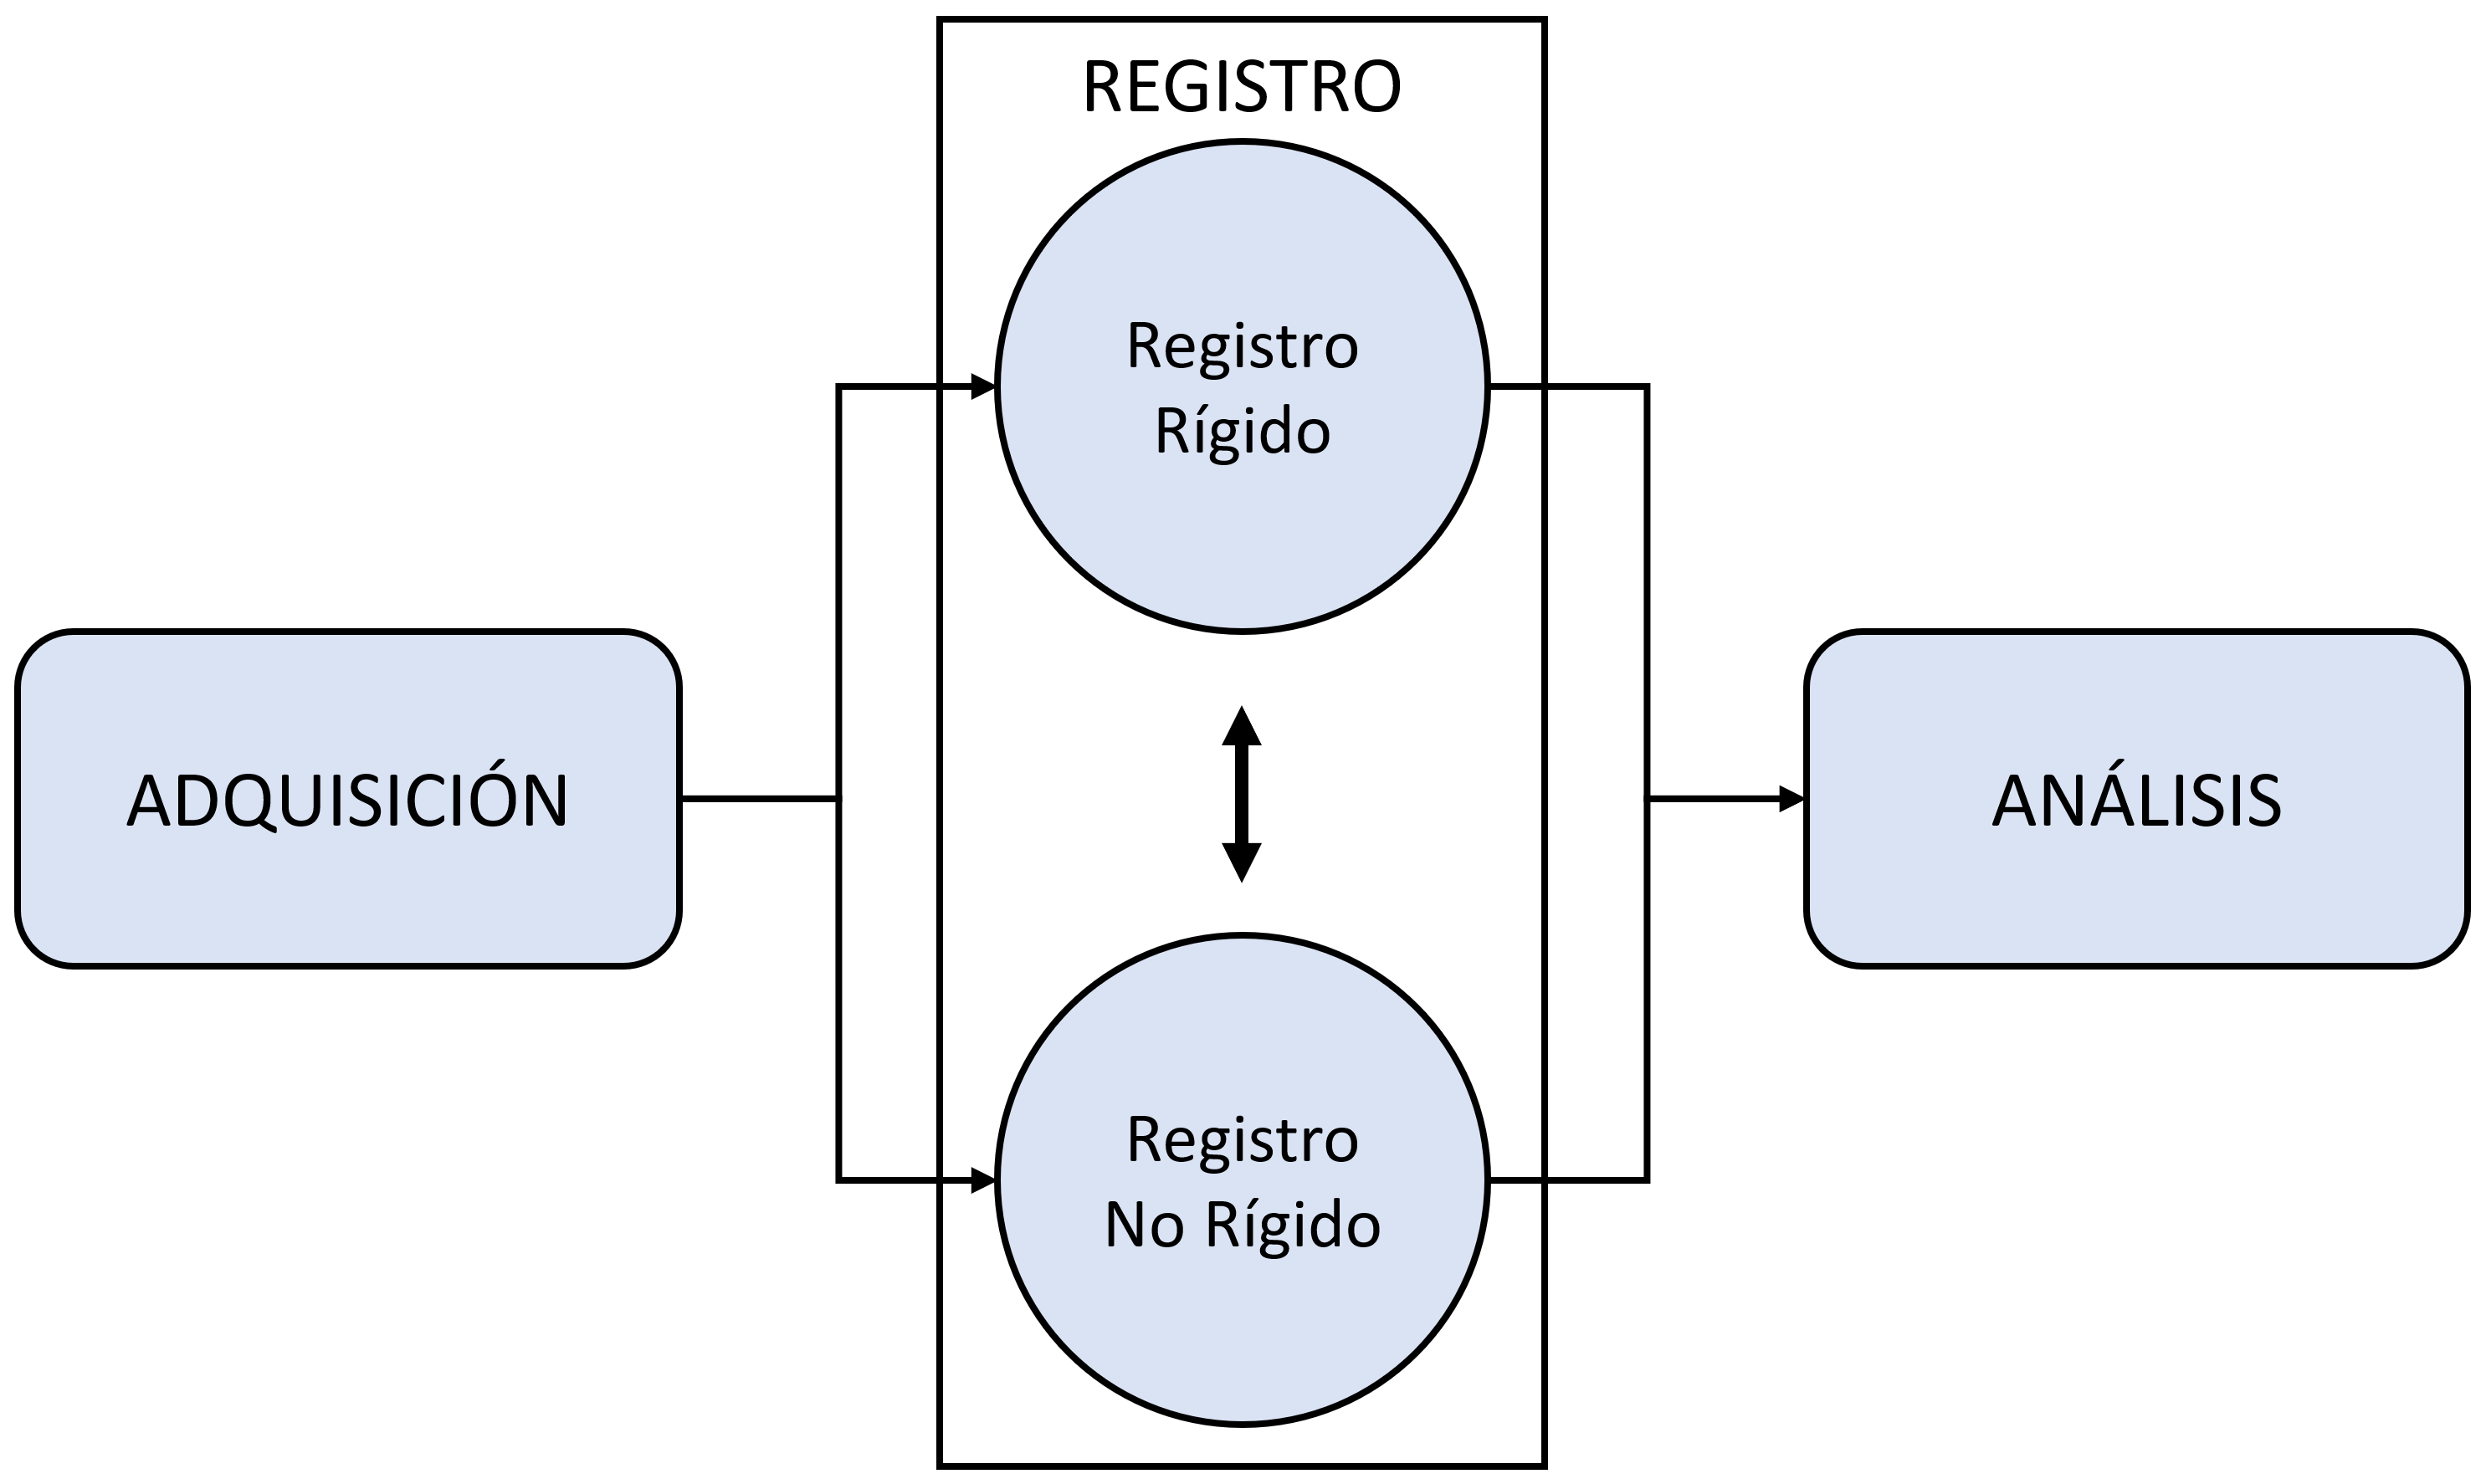
\includegraphics[height=6cm]{archivos/adquisicion-registro-analisis.png}
    \caption{Esquema general de un sistema \glsentryshort{3d}.}
    \label{fig:adquisicion-registro-analisis}
\end{figure}

La adquisición es la primera de las fases para obtener el análisis de una escena.
En esta fase inicial es donde se toman los datos de entrada, por tanto, es la parte del proceso donde interviene el sensor utilizado.
Esta es una parte crítica del sistema, debido a que el resultado de las fases posteriores depende por completo de los datos adquiridos.

% La adquisición de los datos de entrada depende de tres factores principales:
% parámetros del entorno, parámetros del motivo y parámetros de la cámara.
% Los parámetros de entorno hacen referencia al estado en el que se encuentra el entorno, luminosidad, sombras, etc.
% Los parámetros de motivo se refieren a los colores que hay sobre la escena, debido a que el sensor puede estar proyectando colores sobre esta para determinar la profundidad y si coinciden podría dificultar la obtención de los datos.
% Los parámetros de la cámara son los referentes al apartado técnico de la misma:
% la distancia focal, el punto principal, las distorsiones ópticas, el tamaño del sensor, etc.

Tras obtener los datos de entrada en la fase de adquisición, la fase del registro se encarga de realizar las transformaciones necesarias para obtener un modelo completo de la escena.
Existen dos tipos principales de registro:
registro rígido y registro no rígido.
El registro rígido transforma todos los datos al unísono para llevarlos a un mismo sistema de coordenadas, el registro no rígido permite alinear los datos de forma independiente.
Este último es útil para analizar cambios de forma o de color dependiendo del espacio que se esté analizando.

En la última fase, el análisis, se extrae la información necesaria de los datos obtenidos y procesados para cumplir el propósito del problema original.
Este propósito será el que define los requerimientos para la fase de adquisición y de registro.

Por ejemplo, si la escena a analizar se trata de un objeto encima de una mesa, el proceso podría ser obtener los datos desde distintos puntos de vista como primer paso (fase de adquisición).
Seguidamente registrar todas las vistas para que formen el modelo \gls{3d} completo (fase de registro).
Finalmente, el análisis del modelo \gls{3d} nos permite obtener datos útiles de la reconstrucción, como la altura, el volumen, los colores, la forma, etc (fase de análisis).

Habitualmente se asume que los sensores están calibrados para mejorar la adquisición, y el registro de los datos \gls{3d} permita una mejor precisión y exactitud en la fase del análisis.

\section{Estado del arte}
\label{introduccion-estado-arte}

Para abordar este proyecto construyendo un sistema embebido, portable y a la vez económico, se han explorado los diferentes dispositivos que existen en el mercado necesarios para abarcar las diferentes fases del sistema que pretendemos crear.
Es decir, estudiaremos por una parte los diferentes sensores que hay en el mercado para la adquisición de los datos, y por otra parte el hardware necesario que se encargará del registro y del análisis de estos datos.
Además, analizaremos la situación social actual para entender qué necesidades existen y la utilidad que aporta un sistema como el que se pretende construir.
Por último, se hará una pequeña investigación sobre proyectos similares para entender cuál es el estado actual de la tecnología y qué posibilidades ofrece.

\subsection{Hardware para adquisición de datos}
La fase de adquisición depende por completo del sensor utilizado para ello.
Por tanto, es necesario analizar los distintos tipos de sensores para determinar qué sensor será utilizado para dicha finalidad.

% Existen diversos tipos de sensores, y estos se pueden diferenciar principalmente en dos grupos:
% sensores de contacto y sensores sin contacto.

% Los sensores de contacto obtienen la información \gls{3d} de un objeto a través del contacto directo con el mismo.
% Sin embargo, los sensores sin contacto son capaces de obtener esta información desde la distancia.
% Estos últimos suelen ser más rápidos y proporcionan datos adicionales como el color.

Los sensores \gls{3d} pueden diferenciarse en las siguientes categorías:
\gls{lidar}, \gls{tof}, cámaras estereoscópicas y luz estructurada.

\begin{description}
    \item[\gls{lidar}:]
    
    Los sensores \gls{lidar} proyectan un láser en la escena y analizan la reflexión para determinar la distancia y obtener un mapa de profundidad.

    \item[\gls{tof}:]
    
    Los sensores \textit{\glsentrylong{tof}} o ``Tiempo de Vuelo'' en español también proyectan un haz de luz, pero en este caso analizan el tiempo transcurrido entre la emisión y el retorno de dicho haz de luz para determinar la distancia.
    
    A diferencia de los \gls{lidar}, no utilizan un solo pulso de disparo, sino que emiten un cono de disparos, obteniendo información sobre todos los píxeles de la imagen.
    Los escenarios con objetos poco reflectantes pueden tener un impacto negativo en las mediciones realizadas con esta tecnología.
    
    \item[Luz estructurada:]
    
    Los sensores de luz estructurada proyectan un patrón conocido en la escena y calculan la disparidad entre el patrón observado y el conocido.
    Dependiendo del tipo de cámara, puede utilizar patrones codificados temporal o espacialmente.

    Las cámaras de luz estructurada con patrones codificados temporalmente utilizan más de un patrón para crear la imagen y diferenciar los elementos visuales.
    Sin embargo, este enfoque requiere sincronización entre el proyector de patrones y la cámara. 
    
    Por otro lado, las cámaras con patrones codificados espacialmente utilizan similitudes de vecindad espacial y no requieren patrones múltiples.
    No obstante, esta técnica puede presentar problemas en bordes o si hay oclusión del objeto en relación al proyector.

    La iluminación del entorno, así como el motivo, pueden dificultar la identificación del patrón.
    Una vez identificado el patrón, se puede determinar la distancia entre el objeto y la cámara.
    Para ello, es necesario analizar las deformaciones que sufre el patrón sobre la superficie del objeto.

    \item[Cámaras estereoscópicas:]
    
    Las cámaras estereoscópicas consisten en utilizar más de una cámara calibrada en diferentes posiciones para estimar la profundidad calculando la disparidad entre las imágenes obtenidas por cada cámara.

    Se basan en una técnica que utiliza el desplazamiento espacial entre un par de imágenes para triangular y calcular la distancia real entre los objetos y la cámara.
    Muchos sistemas utilizan algoritmos de extracción de características y pueden presentar algunos problemas al intentar identificar puntos clave en escenarios con texturas deficientes.

    A diferencia de los sensores mencionados anteriormente, estos son capaces de proporcionar información de color, pero es necesario calibrar ambos sensores cada vez que varíe su emplazamiento, por tanto, son sensores poco portables.

\end{description}

Los sensores \gls{rgbd} son sensores de propósito general y comúnmente conocidos por su ``bajo coste''.
Combinan las diferentes técnicas de los sensores anteriores con cámaras de color que permiten obtener de forma simultánea la profundidad y el color de la escena.
A través de un sensor \gls{rgbd} podemos obtener un modelo \gls{3d} de un objeto a través de múltiples vistas rotando alrededor del mismo.

En la Figura \ref{fig:d435-sensors} podemos ver un ejemplo de sensor \gls{rgbd}, la Intel RealSense D435.
Este sensor utiliza cámaras estereoscópicas (``Right Imager'' y ``Left Imager'') acompañadas de un proyector \gls{ir} que se encuentra en medio de estas.
El proyector \gls{ir} es una fuente de luz que sirve para iluminar la escena proyectando un patrón de puntos que ayuda a identificar puntos comunes entre las cámaras estereoscópicas.
Estos tres componentes se encargan de capturar la profundidad y están acompañados de un módulo \gls{rgb} para poder capturar la información del color.

\begin{figure}[h]
    \centering
    \begin{subfigure}{0.4\textwidth}
    	\centering
        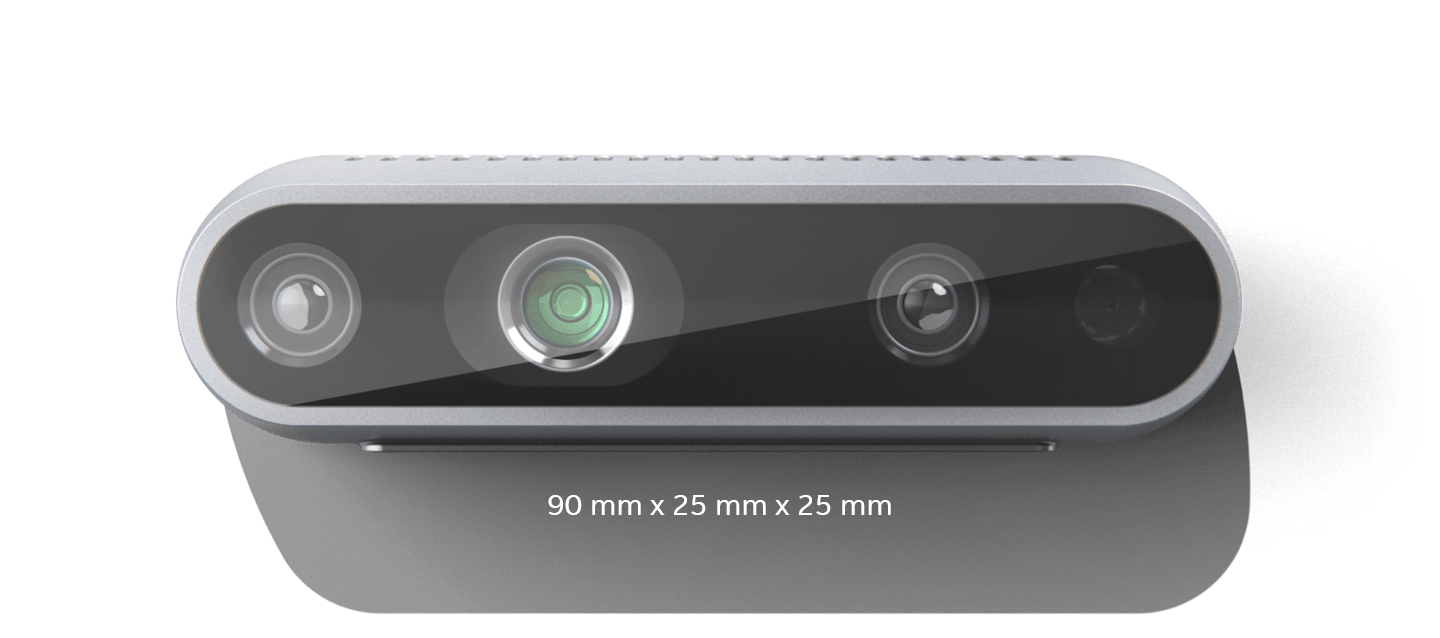
\includegraphics[width=\textwidth]{archivos/d435_image.png}
    \end{subfigure}
    \begin{subfigure}{0.5\textwidth}
    	\centering
        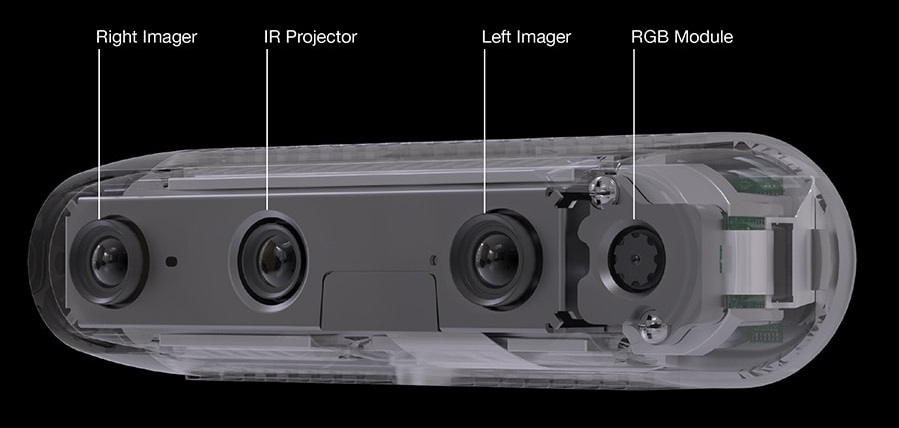
\includegraphics[width=\textwidth]{archivos/d435_sensors.jpg}
    \end{subfigure}
    \caption{Sensor Intel RealSense D435.}
    \label{fig:d435-sensors}
\end{figure}

Como hemos visto, existen diversas categorías de cámaras \gls{3d} con diferentes tecnologías para capturar objetos.
En ``Comparison of RGB-D sensors for 3D reconstruction'' \citep{DaSilvaNeto2020} han realizado una comparación con 10 cámaras \gls{rgbd} de bajo coste distintas para concluir cuáles son las que presentan mejores resultados.

En la Figura \ref{fig:comparacion-sensores-media-error} podemos ver como resultado la media de error obtenida para los 3 recorridos que se han hecho en cada cámara.

\begin{figure}[h]
    \centering
    \begin{subfigure}[b]{0.35\textheight}
    	\centering
        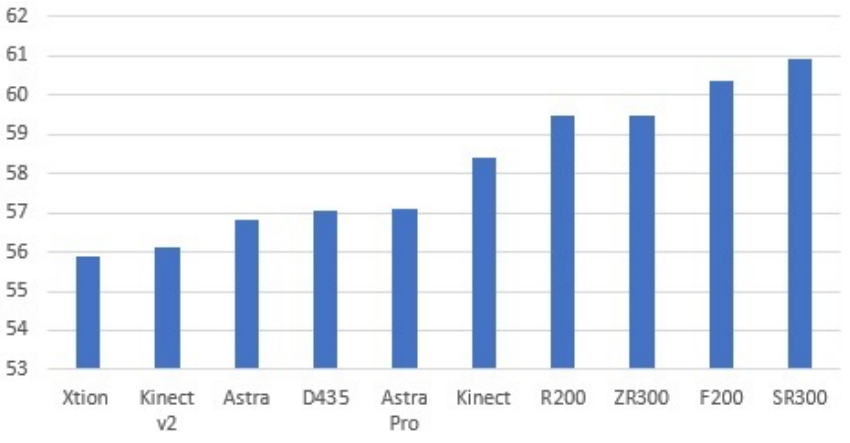
\includegraphics[height=3.5cm]{archivos/comparacion-sensores-recorrido1.png}
        \caption{Ruta 1. Giro simple de 360º.}
        \label{fig:comparacion-ruta1}
    \end{subfigure}
    \begin{subfigure}[b]{0.35\textheight}
    	\centering
        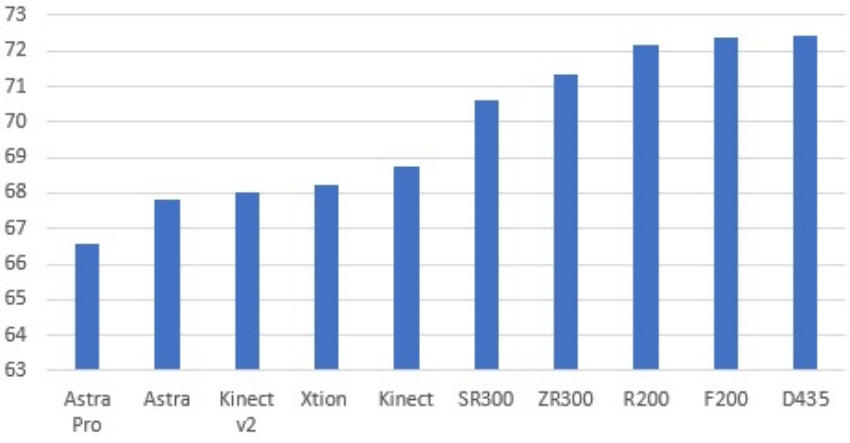
\includegraphics[height=3.5cm]{archivos/comparacion-sensores-recorrido2.png}
        \caption{Ruta 2. Giro de movimiento ondulado.}
        \label{fig:comparacion-ruta2}
    \end{subfigure}
    \begin{subfigure}[b]{0.35\textheight}
    	\centering
        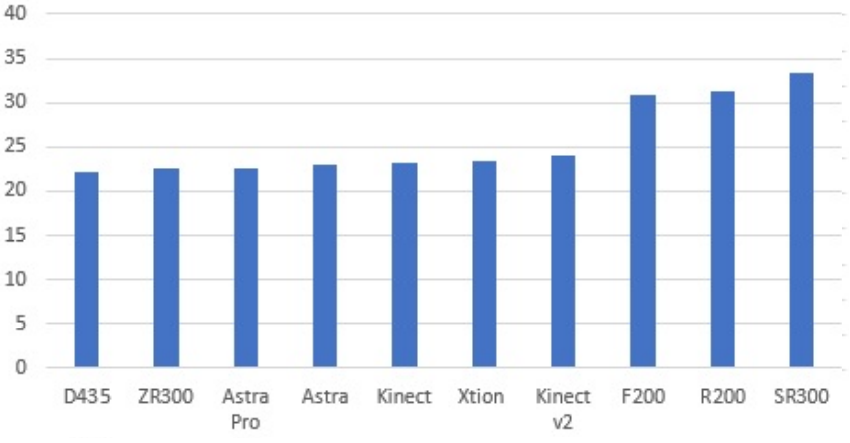
\includegraphics[height=3.5cm]{archivos/comparacion-sensores-recorrido3.png}
        \caption{Ruta 3. Giro cambiando distancia hacia las paredes (acercándose y alejándose).}
        \label{fig:comparacion-ruta3}
    \end{subfigure}
    \caption{Media de error en la comparación de sensores \glsentryshort{rgbd}.}
    \label{fig:comparacion-sensores-media-error}
\end{figure}

% En cada una de las rutas se realiza un giro con la cámara alrededor de la habitación para obtener los datos y recontruirla posteriormente.
% La ruta 1 realiza un giro simple de 360º alrededor de la habitación, la ruta 2 realiza el mismo giro pero con un movimiento ondulado y finalmente la ruta 3 realiza un giro acercandose y alejandose a los objetos.

En general, el Intel D435 obtiene resultados aceptables en las rutas 1 y 3, que son las más similares al caso que abordaremos en este \gls{tfg}.

La prueba donde más destaca el Intel RealSense D435 es en la ruta 3, Figura \ref{fig:comparacion-ruta3}, donde la cámara realiza acercamientos a los objetos.
Esto indica que esta cámara trabaja mejor en escenarios donde la cámara se posiciona cerca del objeto o cuerpo a escanear, lo cual corresponde al objetivo de este \gls{tfg}.

Además, la Intel RealSense D435 se trata del mismo sensor que se utiliza en el proyecto \cite{Tech4DietResultados} del que se ha hablado en la sección \ref{introduccion-motivacion-contexto} de Motivación y Contexto.
Por tanto, este será el sensor a utilizar en este trabajo.

\subsection{Hardware para el registro y análisis de los datos}

Para cumplir con el apartado de registro y análisis de los datos necesitaremos hacer uso de un computador que nos permita:
por una parte almacenar y realizar las modificaciones necesarias a los datos de entrada;
y por otra parte analizar y extraer la información necesaria para el propósito del problema.

Uno de los requisitos que nos proponemos en este proyecto es la capacidad de realizar esto con un dispositivo que sea económico y a la vez portable.
Para ello, se han explorado distintas opciones, como:

\begin{description}
    \item[Raspberry Pi 4 Model B:]
    
    se trata del último modelo de la serie Raspberry Pi. La Raspberry es un mini computador construido en un sistema embebido con un rendimiento comparable con el de un ordenador de sobremesa personal de gama baja.
    
    Estos dispositivos se pueden utilizar como pequeños ordenadores debido a su gran potencial.
    También tiene la capacidad suficiente para usarse como servidor personal por ejemplo.

    Comparado con la anterior generación (Raspberry Pi 3 Model B+) ofrece un aumento significativo en la velocidad del procesador, memoria y conectividad.

    Cuenta con una \gls{cpu} Quad-Core ARM Cortex-A72 de 64 bits a 1.5 GHz de velocidad.
    En cuanto a la \gls{gpu}, cuenta con el chip Broadcom VideoCore VI, con una velocidad de 500 MHz.
    La capacidad de memoria \gls{ram} es de 8 GB LPDDR4 y cuenta con todo tipo de conexiones (USB tipo C, USB Tipo B, microHDMI, conector para cámara\dots).
    
    Con estas especificaciones consigue una potencia computacional de 13.5 GFlops.
    El precio de mercado de este dispositivo está alrededor de 35,00€\footnote{\label{fn:price}El precio indicado se trata del \gls{pvp} oficial recomendado por los fabricantes. Debido a la carencia de chips durante el año 2022 estos precios no se corresponden con la realidad, pudiendo encontrar estos productos por precios mucho más elevados o incluso no quedar stock de los mismos.}.

    \item[Nvidia Jetson Nano:]
    
    la Jetson Nano es la gama de entrada de la familia de Nvidia Jetson.
    Nvidia Jetson es una serie de computadores embebidos, parecidas a las Raspberrys pero con \gls{gpu}s más potentes.
    Esto nos permitirá realizar operaciones en paralelo en algoritmos para la visión por computador.

    Cuenta con una \gls{cpu} Quad-Core ARM Cortex-A57 de 64 bits a 1.42 GHz de velocidad.
    En cuanto a la \gls{gpu}, el chip está basado en la arquitectura Maxwell de Nvidia, cuenta con 128 \gls{cuda} cores con una velocidad de 921 MHz.
    La capacidad de memoria \gls{ram} es de 4 GB LPDDR4 y cuenta con todo tipo de conexiones (USB tipo C, USB Tipo B, microHDMI, conector para cámara\dots).

    Con estas especificaciones consigue una potencia computacional de 472 GFlops.
    El precio de mercado de este dispositivo está alrededor de 89,00€\footref{fn:price}.

    \item[Nvidia Jetson TX2:]
    
    se trata de un modelo superior a la Jetson Nano, con especificaciones superiores, pero también más caro.

    Cuenta con una \gls{cpu} Quad-Core ARM Cortex-A57 de 64 bits a 2.00 GHz de velocidad.
    En cuanto a la \gls{gpu}, el chip está basado en la arquitectura Pascal de Nvidia, cuenta con 256 \gls{cuda} cores con una velocidad de 1300 MHz.
    La capacidad de memoria \gls{ram} es de 8 GB LPDDR4 y cuenta con todo tipo de conexiones (USB tipo C, USB Tipo B, microHDMI, conector para cámara\dots).

    Con estas especificaciones consigue una potencia computacional de 1.3 TFlops.
    El precio de mercado de este dispositivo está alrededor de 399,00€\footref{fn:price}.
\end{description}

Como podemos observar, la Nvidia Jetson Nano cuenta con un procesador ligeramente inferior al de la Raspberry Pi 4 Model B.
Sin embargo, la \gls{gpu} es mucho más potente, con 128 núcleos a 921 MHz que permite superar en potencia computacional a la Raspberry unas 35 veces.

Además, nuestro proyecto trabaja con la visión por computadores, lo cual quiere decir que se realizará un gran número de operaciones y cálculos fácilmente paralelizables.
Para poder sacar mejor rendimiento y aprovechar la concurrencia de los cálculos, viene bien hacer uso de una \gls{gpu} con muchos núcleos, por tanto será necesario una \gls{gpu} más potente que el chip que incluye la Raspberry Pi 4 Model B.

Por otro lado, la Nvidia Jetson TX2 es claramente superior en especificaciones a la Nvidia Jetson Nano.
Cuenta con un procesador un poco más potente y una \gls{gpu} con el doble de núcleos a 1300 MHz de velocidad, superando en potencia computacional casi 3 veces a la Jetson Nano, pero con un precio muy superior.

``Benchmark Analysis of Jetson TX2, Jetson Nano and Raspberry PI using Deep-CNN''
\citep{Suzen2020} se trata de una investigación donde miden el rendimiento de estos tres dispositivos para aplicaciones que usan deep learning. Si bien nuestro proyecto de investigación no se basa en el deep learning, el principio para determinar el rendimiento de estos dispositivos es el mismo, la concurrencia.

En el estudio de \cite{Suzen2020} utilizan 5 conjuntos de datos de varios tamaños.
En la Figura \ref{fig:resultados-benchmark-tx2-nano-raspberry} se ve que hay un error de memoria para la Nvidia Jetson Nano y la Raspberry Pi.
No es un problema que deba preocuparnos ya que esto es un problema que surge cuando se requiere de un conjunto tan grande de datos para el deep learning.
Para nuestro proyecto, basado en la visión por computador, no será un límite a tener en cuenta.

También podemos ver el resultado del estudio, con el porcentaje de aciertos, el tiempo que emplean, la memoria utilizada y el consumo.
Para nuestro caso, el resultado de mayor interés a tener en cuenta es el tiempo, ya que es la forma de medir qué dispositivo tiene un mejor rendimiento.

\begin{figure}[h]
    \centering
    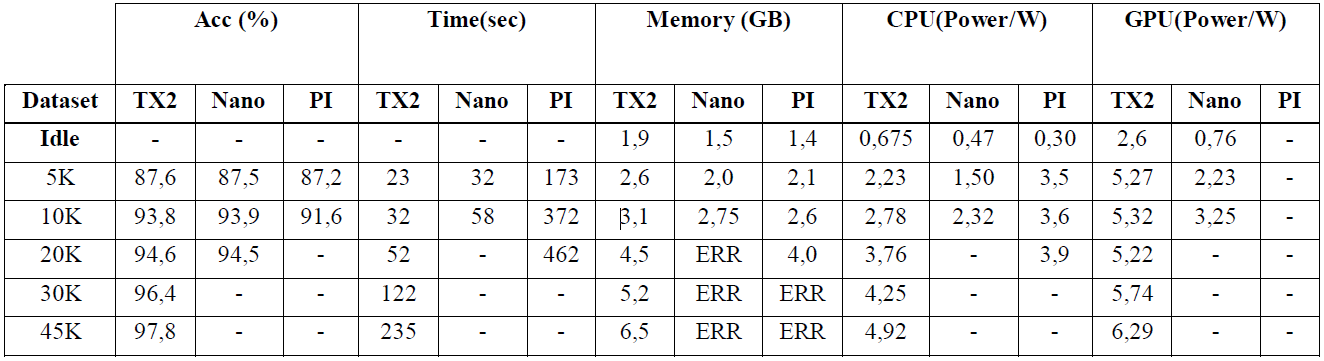
\includegraphics[width=\linewidth]{archivos/resultados-benchmark-tx2-nano-raspberry.png}
    \caption{Benchmarking Nvidia Jetson TX2, Nvidia Jetson Nano y Raspberry Pi 4 Model B.}
    \label{fig:resultados-benchmark-tx2-nano-raspberry}
\end{figure}

Como podemos ver, las Nvidia Jetson quedan muy por encima de la Raspberry Pi 4 Model B, con unos resultados muy parecidos entre ellas, siendo superior la Nvidia Jetson TX2 en todos los casos.

Aunque la Nvidia Jetson TX2 es la clara ganadora en rendimiento, para este proyecto la potencia no lo es todo.
Entre nuestros requisitos para construir el escáner \gls{3d}, los dispositivos a utilizar deben ser portables y económicos. Los 3 computadores que hemos comparado son igual de portables, pero la Jetson TX2 tiene un precio demasiado elevado para el coste económico que estamos buscando.

Para poder comparar la calidad/precio de cada uno de los dispositivos, nos fijaremos en la potencia computacional para medir la calidad de los mismos.
Por tanto, nos centraremos en el precio del GFlop en cada uno de los dispositivos.
Podemos ver que en la Raspberry Pi 4 Model B tendría un coste de 2,60€/GFlop, la Nvidia Jetson Nano un coste de 0,19€/GFlop y la Nvidia Jetson TX2 un coste de 0,30€/GFlop.

Además, si nos basamos en los resultados de los benchmarks que se muestran en la Figura \ref{fig:resultados-benchmark-tx2-nano-raspberry}, la diferencia de rendimiento en tiempo entre la Nvidia Jetson Nano y la Nvidia Jetson TX2 no es tan grande como para compensar el coste económico que supone hacerse con una Nvidia Jetson TX2.

Por tanto, la opción más recomendable para este proyecto es, sin lugar a dudas, la Nvidia Jetson Nano, que nos ofrece un rendimiento aceptable, muy superior a una Raspberry PI y por un precio muy económico.

% No obstante, hay que tener en cuenta que no es comparable el rendimiento que estos computadores embebidos pueden proporcionar frente a sobremesas que cuentan con una \gls{gpu} dedicada.

% Como podemos ver en ``Benchmarking GPU-Accelerated Edge Devices'' \citep{Jo2020}, otro estudio sobre el uso de \gls{gpu} para deep learning, las Nvidia Jetson Nano y TX2 son capaces de completar los benchmarks eficientemente.
% No obstante, no son comparables con el rendimiento de \gls{gpu}s como la GTX 1060 o la Tesla V100, gráficas dedicadas que han utilizado en los benchmarks de la investigación.
% En estos benchmarks se demuestra que para procesos o aplicaciones demasiado complejas los computadores embebidos pueden ser insuficientes.

% Para el propósito de este proyecto, el rendimiento que nos proporcionará la Nvidia Jetson Nano es suficiente.

\subsection{Situación social actual, necesidades y aplicaciones}

Un escáner \gls{3d} tiene la capacidad de analizar un objeto o una escena para reunir datos sobre su forma y, ocasionalmente, su color.
Con la información obtenida se puede pasar a construir modelos digitales tridimensionales.

Al principio, las utilidades y aplicaciones que proporcionaba esta tecnología era utilizada exclusivamente en el ámbito industrial.
Hoy en día, gracias a los avances y a la popularidad de la tecnología, es utilizada en una amplia variedad de actividades, tales como arquitectura, ingeniería, medicina, arqueología y entretenimiento, entre otras.
A continuación, comentaré algunos ejemplos de ellos. Veremos como son muchas las utilidades que un escáner \gls{3d} ofrece, y que existe la necesidad de herramientas así que sean portables y de bajo coste.

En el ámbito industrial e ingenieril tiene diferentes aplicaciones debido a su gran capacidad para capturar de forma rápida y precisa los datos requeridos.
De otra forma, las mediciones tendrían que ser recolectadas por métodos manuales que pueden ser menos exactos, muy costosos y consumir mucho tiempo.
Como por ejemplo se estudia en el artículo ``Generación de prototipos por modelado, escaneado e impresión 3D'' \citep{RayonEncinas2015} de la \gls{upv} donde desarrollan una metodología docente enfocada a los alumnos de \gls{ididp} para el uso del escáner \gls{3d}. En este informe dan a conocer la importancia y necesidad del escáner \gls{3d}, donde digitalizan un objeto en \gls{3d} y realizan modificaciones en el diseño para finalmente generar un prototipo real por impresión \gls{3d}, facilitando así el desarrollo de un producto.

En el ámbito de la salud más cercano a la temática del proyecto los requerimientos de escaneo \gls{3d} son diversos, como explican en el artículo científico ``3D scanning applications in medical field: A literature-based review'' \citep{Haleem2019} donde hablan de la importancia de esta tecnología y del crecimiento que ha tenido en el campo de la medicina en los últimos años.
Por ejemplo, los profesionales de la salud pueden de forma muy rápida realizar un escaneo corporal completo, facilitando así la obtención y comparación de datos precisos para llevar a cabo investigaciones y monitorizar los cambios en las mediciones corporales que ocurren con el tiempo.
Esto es posible gracias a investigaciones como las que se han hecho en \cite{Tech4DietResultados}, con artículos científicos como ``RGB-D-Based Framework to Acquire, Visualize and Measure the Human Body for Dietetic Treatments'' \citep{Fuster-Guillo2020}.

Por otro lado, el escaneo \gls{3d} también trae la posibilidad de crear soluciones personalizadas para el cuidado de la salud.
Por ejemplo, en ``Reconstrucción digital del muñón de un amputado transfemoral a partir de datos obtenidos de escáner 3D'' \citep{isaza2011reconstruccion} muestran como el uso de un escáner \gls{3d} permite realizar reconstrucciones sobre un molde tomado de un muñón.
``Diseño de prótesis inferiores impresas en 3D para personas amputadas en Camerún'' \citep{martinez2020diseno} es otro ejemplo donde muestran el desarrollo del proceso de diseño de prótesis inferiores, haciendo uso de técnicas de digitalización e impresión \gls{3d}, debido a que es rápida, económica y permite la personalización de las prótesis para cada paciente.

En el ámbito de la medicina forense también se está experimentando un crecimiento en el uso de técnicas \gls{3d}.
Ofrecen portabilidad, flexibilidad y precisión que facilita la tarea de recopilar datos forenses comparado con los métodos tradicionales.
Por ejemplo, en la investigación ``Geotecnologías láser y fotogramétricas aplicadas a la modelización 3D de escenarios complejos en infografía forense'' \citep{blazquez2015geotecnologias} proponen el uso de escáneres \gls{3d} para la identificación por superposición craneofacial.
Para ello, utilizan una plataforma giratoria que automatiza la adquisición de las distintas vistas del cráneo para aumentar la rapidez y precisión de la obtención del modelo \gls{3d}.
Un concepto muy parecido al que se desea realizar en este trabajo.

Por último, en el ámbito de la paleontología y arqueología gracias a las tecnologías \gls{3d} se ha conseguido la creación de réplicas digitales de gran precisión de diversos artefactos, desde la recreación de elementos encontrados durante excavaciones hasta la creación de museos online con cientos de exhibiciones.
En ``Restauración y conservación digital de fósiles mediante escaneado 3D y la reproducción con prototipado rápido'' \citep{Valverde-Bastidas2020} se utiliza ingeniería inversa mediante el escaneado \gls{3d} para obtener una nube de puntos en tres dimensiones de un objeto material.
Posteriormente tratan esa malla para luego realizar una reingeniería, un rediseño o directamente para volver a fabricar el objeto.

\subsection{Investigaciones y otros proyectos ya realizados}

Se han investigado proyectos cuyo hardware es parecido al que se pretende utilizar en este trabajo de investigación.
En ``Analysis of 3D perception based on depth sensors in order to perform 3D scene understanding'' \citep{fioriti2021analysis} pretenden realizar un análisis de las características de percepción 3D con la ayuda de sensores de profundidad.
Para ello han utilizado una cámara \gls{rgbd} Intel RealSense D435 conectada inicialmente a una Raspberry Pi 3, utilizando el algoritmo de detección Yolo adaptado para usar una detección \gls{3d}.
De esta forma, han implementado un sistema capaz de detectar la distancia que hay con el objeto.
El algoritmo puede ser utilizado tanto con imágenes como con un vídeo del objeto.
El problema actual que tienen es que no puede ser utilizado en tiempo real, pues para ello necesitan acelerar el proceso.
Esto es debido seguramente a las bajas prestaciones del hardware, ya que utilizan una Raspberry Pi 3 cuya \gls{gpu} es muy pobre comparada con la \gls{gpu} de la Nvidia Jetson Nano que utilizaremos en este proyecto.

En ``Development of augmented reality systems displaying three-dimensional
dynamic motion in real time'' \citep{Aoki2020} han utilizado también el sensor D435 conectado a un dispositivo Raspberry Pi 4.
Con este hardware pretenden desarrollar un sistema de seguimiento de un movimiento tridimensional mostrando en tiempo real la trayectoria en un dispositivo móvil.
Por tanto, han desarrollado una aplicación para poder seguir objetos \gls{3d} con el sensor y mostrar la trayectoria en realidad aumentada desde el dispositivo móvil.
Esta aplicación tiene una limitación respecto a la velocidad del movimiento, ya que la frecuencia del muestreo ha sido limitada a 8 fps debido a las especificaciones del hardware.
De nuevo, esto se podría solucionar utilizando un hardware más potente como la Nvidia Jetson Nano, que permitiría paralelizar gran parte del proceso aumentando la frecuencia del muestreo máxima y permitiendo así detectar movimientos más rápidos.

\section{Objetivos}
\label{introduccion-objetivos}

El objetivo general es proponer una arquitectura de visión por computador que sea capaz de modelar en \gls{3d} objetos deformables. Concretamente, para este \gls{tfg} el objetivo principal es hacer un sistema embebido de bajo coste que permita modelar un cuerpo o individuo articulado, como lo es un cuerpo humano.
Para ello, se plantean tres subobjetivos:

\begin{itemize}
    \item El primer subobjetivo es realizar un análisis del estado del arte para evaluar la situación en la que nos encontramos. Además, se analizarán las tecnologías y herramientas necesarias para llevar a cabo el objetivo del proyecto.
    \item Hacer una propuesta de solución. Este subobjetivo consistirá en integrar el SDK del sensor \gls{rgbd} Intel RealSense D435 con el dispositivo Nvidia Jetson Nano, implementar una solución, validarla y documentarla.
    \item Por último, experimentar y estudiar los resultados obtenidos.
\end{itemize}

\section{Desarrollo de la memoria}
\label{introduccion-desarrollo}

A continuación, los siguientes capítulos contendrán las bases teóricas y el desarrollo del tema principal del trabajo.
Está organizado de la siguiente manera:

El capítulo \ref{cap:base-teorica} nos presenta la base teórica necesaria para comprender el desarrollo e investigación que se ha llevado a cabo a lo largo del proyecto.

El capítulo \ref{cap:realsense-d435} habla del sensor Intel RealSense Depth Camera D435.
En este capítulo se analiza más detalladamente el funcionamiento y las características de este sensor, que es el utilizado en este trabajo.

El capítulo \ref{cap:propuesta-de-solucion} muestra la propuesta del trabajo, explicando detalladamente los pasos que se van a seguir para obtener una solución a la reconstrucción de un cuerpo humano utilizando el sensor Intel RealSense D435 y el sistema embebido Jetson Nano.

En el capítulo \ref{cap:solucion-proyecto} explica cómo se ha llevado a cabo la propuesta del capítulo anterior, mostrando fragmentos de código y la solución final obtenida.

Seguidamente en el capítulo \ref{cap:experimentacion} se mostrarán los resultados que se obtienen con la solución del proyecto.

Finalmente, en el capítulo \ref{cap:conclusion} nos encontraremos con la conclusión del trabajo elaborado en este proyecto.
